\documentclass[10pt]{report}
\usepackage[utf8]{inputenc}
\usepackage[T1]{fontenc}
\usepackage[english]{babel}
\usepackage{fourier} % Nicenesss font
\usepackage{amsfonts,amsmath}
\usepackage[pdftex]{color,graphicx}
\usepackage{pdfpages}
\usepackage{fancyhdr}
\usepackage{textcomp}
\usepackage{lmodern}
\usepackage{xcolor}
\usepackage{multicol}
\usepackage{soul}
\usepackage{algorithmic}
\usepackage{wrapfig}
\usepackage{float}
\usepackage{mdwlist}
\usepackage{pgfgantt}
\usepackage{a4wide}
\usepackage{tabularx}
\usepackage{booktabs}

\newcommand{\tabitem}{~~\llap{\textbullet}~~}

\usepackage{hyperref}
\usepackage{lscape}

\usepackage{sectsty}
\allsectionsfont{\centering \normalfont\scshape}
\renewcommand{\thesection}{\arabic{section}}

\numberwithin{equation}{section} % Number equations within sections (i.e. 1.1, 1.2, 2.1, 2.2 instead of 1, 2, 3, 4)
\numberwithin{figure}{section} % Number figures within sections (i.e. 1.1, 1.2, 2.1, 2.2 instead of 1, 2, 3, 4)
\numberwithin{table}{section} % Number tables within sections (i.e. 1.1, 1.2, 2.1, 2.2 instead of 1, 2, 3, 4)

%\usepackage{hyperref}
\pagestyle{fancy}
\newcommand{\HRule}{\rule{\linewidth}{0.5mm}}

%If in need of a header for the document, uncomment this and add desired text!
%\fancyhead[LO,LE]{}
%\fancyhead[RO,RE]{}
%

%Macro foo
\newcommand{\method}[3]{ \label{method:#2}
    {\vspace{10pt} \noindent \textbf{#1} \textit{#2}(#3)} :
}
\newcommand{\argument}[2]{{\textbf{#1} #2}}


%%%%%%%%%%%% END OF PREAMBLE %%%%%%%%%%%%%%%%%%%%%%%%%%%%%%%%%%%%
\begin{document}
\begin{titlepage}

\begin{center}

\textsc{\LARGE BDSA}\\[1.5cm]

\textsc{\Large System Design Document}\\[0.5cm]

\HRule \\[0.4cm]

{ \bfseries Assignment \#39 \\[0.5cm] 
    {\small \today}} \\[0.7cm]

\HRule \\ [6.5cm]

% Author and supervisor
\begin{minipage}{0.5\textwidth}
\begin{flushleft} \large
Ahmed Al Aqtash (ahaq)\\
\textit{ahmed.aqtash@gmail.com}\\
Mikkel Åxman (mikx)\\
\textit{mikx@itu.dk}\\
Phillip Phoelich (ppho)\\
\textit{ppho@itu.dk}\\

\vfill 
\end{flushleft}
\end{minipage}
% Bottom of the page front page

\end{center}

\end{titlepage}
\clearpage
\begin{table}[h]
\begin{tabularx}{\textwidth}{l l X l}
\textbf{Version} & \textbf{Date} & \textbf{Description} & \textbf{Authors} \\ \midrule
1.0     & 9/9-2014 & First version of the SDD & ahaq, mikx, ppho \\
\end{tabularx}
\end{table}

\clearpage
%% Generelle struktur %%
\section{Introduction}
This is a breakdown of a simple calendar system, which provides means to
synchronise across multiple clients.

\subsection{Purpose of the system}
The purpose of this system is to provide users with a calendar system they can
use on any PC. In its current form, users can add calendars and events, and
synchronise these to a central server. Users should also be able to share
calendars.

\subsection{Design goals}
\subsubsection{Usability}
\begin{itemize}
\item A User must be able to successfully add a calendar in less than 30
  seconds, typing excluded.
\item A User must be able to add an event in less than 60 seconds, typing
  excluded.
\item A User must be able to add a calendar and publish it in less than 60
  seconds, bandwidth and typing excluded.
\end{itemize}
\subsubsection{Response time}
\begin{itemize}
\item Syncronising a calendar with the server should happen within 5 second,
  excluding differences in internet speeds.
\end{itemize}
\subsubsection{Fault tolerance}
\begin{itemize}
\item If the internet connection is lost, the User must be able to continue
  working. Changes will be syncronised with online calendar on reconnection.
\end{itemize}
\subsubsection{Robustness}
\begin{itemize}
\item An average user cannot give wrong input.
\end{itemize}
\subsubsection{Portability}
\begin{itemize}
\item The system should be able to be accessed from any given platform, running C\#.
\end{itemize}
\subsubsection{Extensibility}
\begin{itemize}
\item The way of storing calendars should be easily exchangeable.
\end{itemize}
%\subsubsection{Reliability}
%\subsubsection{Performance}
%\subsubsection{Supportability}
%\subsubsection{Implementation}
%\subsubsection{Interface}
%\subsubsection{Packaging}
%\subsubsection{Legal}
\subsection{Definitions, acronyms, and abbreviations}
\subsection{References}
\subsection{Overview}

\section{Current software architecture}

\section{Proposed software architecture}
\subsection{Overview}
\subsection{Subsystem decomposition}
\begin{figure}
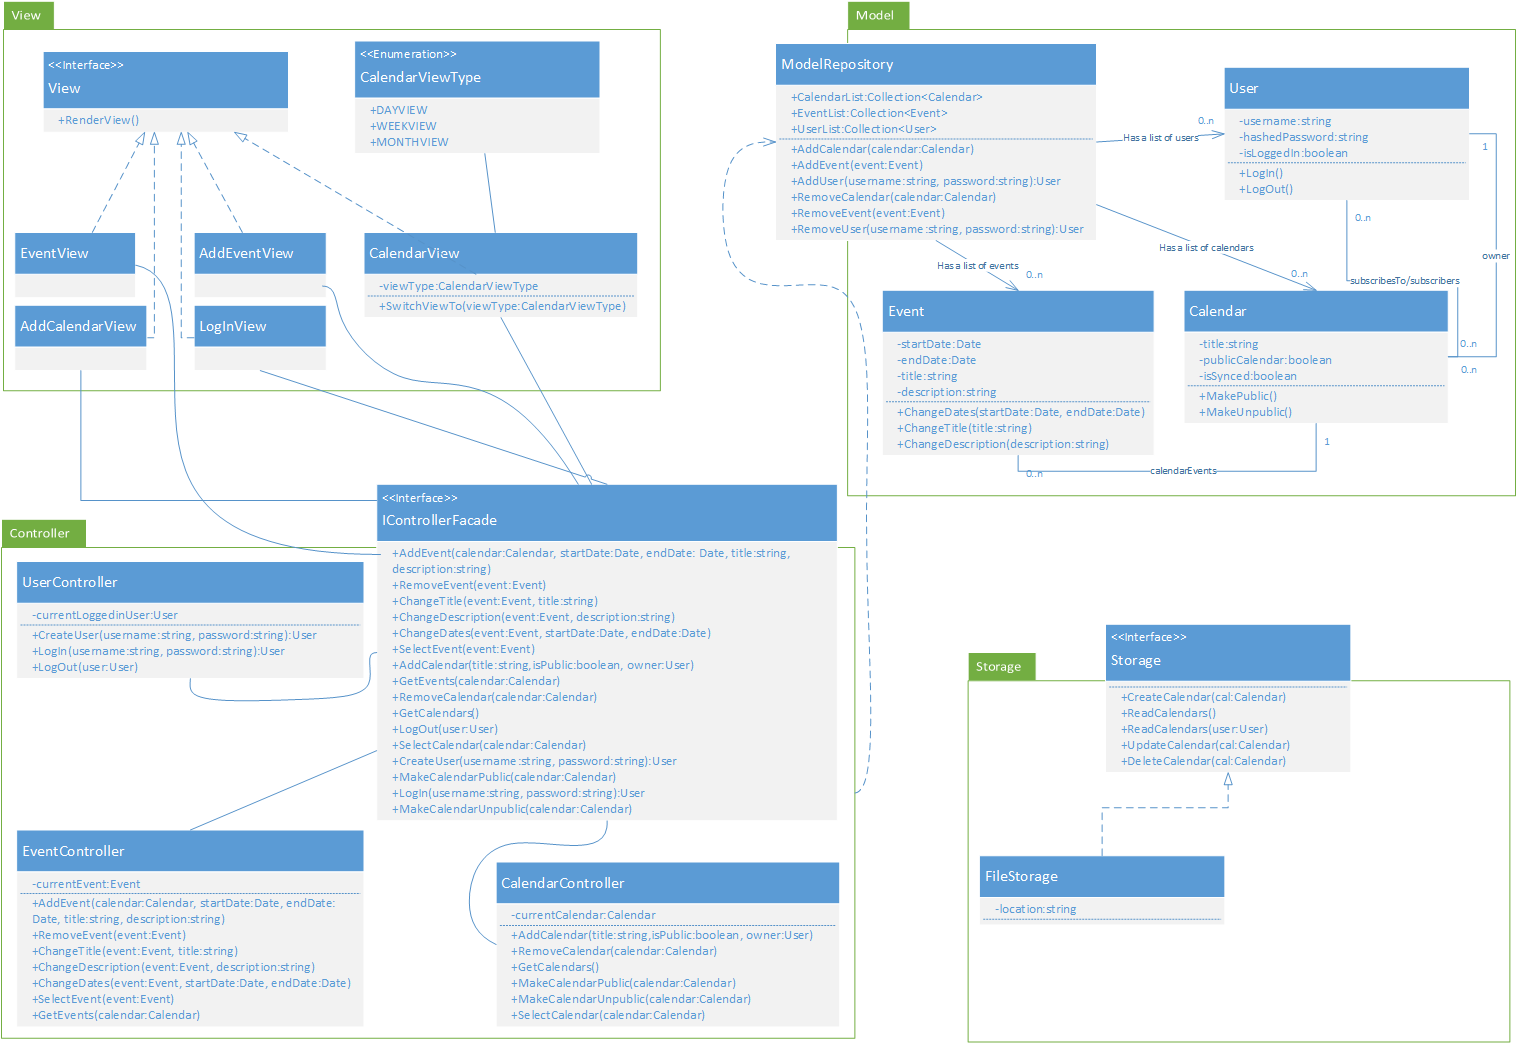
\includegraphics[scale=0.40]{classdiagram.png}
\end{figure}
\subsection{Hardware/software mapping}
\subsection{Persistent data management}
\subsection{Access control and security}
\subsection{Global software control}
\subsection{Boundary conditions}

\section{Subsystem services}

%\section{Glossary}

\end{document}
